% Compilar:  make report   (o LaTeX Workshop -> receta "Docker LuaLaTeX")
% Límite: 12 páginas de cuerpo (resumen ... opinión). Los anexos no cuentan.
\documentclass[11pt]{article}
\newcommand{\CaseId}{B} % <-- caso asignado
% ---------------------------------------------------------------- idioma y fuentes
\usepackage{fontspec}
\setmainfont{Liberation Serif} % clon métrico de Times New Roman (luaotfload no resuelve ese nombre localmente)
\usepackage[spanish,es-nodecimaldot]{babel}

% ---------------------------------------------------------------- página
\usepackage[a4paper,margin=2.5cm]{geometry}
\usepackage{parskip}
\usepackage{microtype}

% ---------------------------------------------------------------- matemáticas
\usepackage{amsmath,amssymb,bm}

% ---------------------------------------------------------------- figuras y tablas
\usepackage{graphicx}
\graphicspath{{figures/}}
\usepackage{booktabs,longtable,array}
\usepackage{caption}
\captionsetup{font=small,labelfont=bf}
\usepackage{float}
\usepackage{xcolor}

% ---------------------------------------------------------------- código y JSON
\usepackage{listings}
\lstset{basicstyle=\ttfamily\footnotesize,breaklines=true,frame=single,columns=fullflexible}

% ---------------------------------------------------------------- bibliografía y enlaces
\usepackage{csquotes}
\usepackage[backend=biber,style=apa]{biblatex}
\addbibresource{references.bib}
\usepackage{hyperref}
\hypersetup{
    colorlinks=true,
    linkcolor=black,
    filecolor=black,
    urlcolor=blue,
    citecolor=black,
    pdftitle={Optimum Investments --- Caso OP01 (Caso \CaseId)}
}
\usepackage{xparse}

% ---------------------------------------------------------------- encabezado y pie de página
\usepackage{fancyhdr}
\setlength{\headheight}{14pt}
\pagestyle{fancy}
\fancyhf{}
\fancyhead[L]{\textbf{Optimum Investments}}
\fancyhead[R]{\textit{Caso OP01 --- Caso \CaseId}}
\fancyfoot[R]{\thepage}
\renewcommand{\headrulewidth}{0.4pt}

% ---------------------------------------------------------------- títulos de sección
\usepackage{titlesec}
\titleformat{\section}[block]
  {\normalfont\bfseries\fontsize{16pt}{18pt}\selectfont\color{black}}
  {\thesection}{0.3em}{}
\titleformat{\subsection}[block]
  {\normalfont\bfseries\fontsize{14pt}{15pt}\selectfont}
  {\thesubsection}{0.2em}{}

% ---------------------------------------------------------------- notación del modelo
\newcommand{\R}{\mathbb{R}}
\newcommand{\E}{\mathbb{E}}
\newcommand{\Var}{\operatorname{Var}}
\newcommand{\CVaR}{\operatorname{CVaR}}
\newcommand{\VaR}{\operatorname{VaR}}
\newcommand{\SigmaF}{\bm{\Sigma}_F}
\newcommand{\SigmaV}{\bm{\Sigma}_V}
\newcommand{\M}{\mathbf{M}}
\newcommand{\PEN}{S/\,}
\newcommand{\PN}{\mathit{PN}}
\newcommand{\todo}[1]{\textcolor{red}{\textbf{[TODO: #1]}}}

% ---------------------------------------------------------------- portada
\NewDocumentCommand{\cover}{mmm}{%
  \begin{titlepage}
    \vspace*{2\baselineskip}
    \begin{center}
        
\includegraphics[height=4.2cm]{EPG.png}
    \end{center}

    \vspace*{4\baselineskip}

    \begin{center}
        \textbf{\uppercase{\fontsize{14pt}{14pt}\selectfont #1}}
    \end{center}

    \vspace*{2\baselineskip}

    \begin{center}
        \textbf{\fontsize{12pt}{12pt}\selectfont #3}
    \end{center}

    \vspace*{4\baselineskip}

    \begin{center}
        \textbf{\fontsize{12pt}{12pt}\selectfont Presentado por}
    \end{center}
    \begin{center}
        \textbf{\fontsize{12pt}{12pt}\selectfont #2}
    \end{center}

    \vfill

    \begin{center}
        \textbf{\fontsize{12pt}{12pt}\selectfont Lima, \today}
    \end{center}
  \end{titlepage}
}


\title{Optimum Investments: optimización de riesgo patrimonial\\[4pt]
       \large Caso OP01 --- Caso \CaseId}
\author{Nombre Apellido}
\date{\today}

\begin{document}
\maketitle
\thispagestyle{empty}

\section{Resumen ejecutivo}\label{sec:resumen}

Optimum Investments cierra 2025 con un patrimonio neto (PN) de \PEN200 mm sobre \PEN1{,}000 mm de activos
y \PEN800 mm de pasivos. Evaluada a un año con la historia de mercado 2021--2025, esa posición inicial
arriesga mucho más de lo que rinde: el resultado esperado es de solo \PEN3.96 mm, pero la volatilidad del
patrimonio es de \PEN25.4 mm y su pérdida esperada en el 5\,\% de escenarios más adversos (CVaR al 95\,\%)
alcanza \PEN50.1 mm, un cuarto del patrimonio. La cartera además incumple el propio límite de renta variable
del banco (22\,\% de los activos contra un máximo de 20\,\%).

Este informe recomienda reestructurar activos y pasivos hacia la cartera que minimiza esa pérdida de cola con
una aversión al riesgo $\lambda = 0.25$: subir la caja en soles a \PEN200 mm, concentrar la renta fija en soles
en el bono A02 (hasta su tope individual de \PEN350 mm), duplicar la posición en el bono flotante en dólares
A05 (a \PEN240 mm), liquidar el bono fijo en dólares A04 y recortar la renta variable a su piso de \PEN50 mm;
del lado de los pasivos, llevar el préstamo corto en soles L01 a su tope de \PEN280 mm y reducir el bono fijo
L02 a \PEN40 mm. Pagando \PEN2.73 mm en costos de transacción, esta cartera baja la volatilidad del patrimonio
a \PEN7.0 mm y el CVaR al 95\,\% a \PEN7.8 mm --- una caída de 84\,\% --- a cambio de solo \PEN0.85 mm de
resultado esperado neto (de \PEN3.96 mm a \PEN3.11 mm).

El principal riesgo de esta recomendación no es de mercado sino de modelo: los cuatro escenarios de estrés del
caso deprecian el sol sin excepción, y sustituir la regla de proyección de cupones flotantes por la forward del
período cambia el resultado de la cartera óptima en el escenario de estrés más severo de \mbox{$-$\PEN18.8 mm} a
\mbox{$-$\PEN5.8 mm} (Sección~\ref{sec:sensibilidad}). Además, el préstamo corto L01 llevado a su tope incumple con
certeza (100\,\% de probabilidad) el límite de vencimientos de corto plazo una vez llegado el horizonte;
exigir ese límite también en el horizonte cuesta \PEN0.29 mm de resultado esperado neto.

\section{Datos y supuestos}\label{sec:datos}
% Balance inicial (Cuadros 1-2), historia 2021-2025 (60 obs.), convenciones de curva,
% definición de cambios de factores, spreads de calibración.
\todo{Describir balance inicial y datos.}

\paragraph{Convenciones.} Tasas spot efectivas anuales; tiempo ACT/365; interpolación
lineal de la tasa cero entre nodos; nodo O/N en $t=0$. Cambios de factores: diferencia
absoluta en tasas y log-retorno en tipo de cambio y renta variable.

% Tabla generada por notebooks/05 con save_table() y figura por notebooks/00 con save_fig().
\begin{table}[htbp]
\centering
\caption{Balance inicial al 31-12-2025}
\label{tab:balance}
\resizebox{\ifdim\width>\textwidth\textwidth\else\width\fi}{!}{%
\begin{tabular}{llllr}
\toprule
 & Lado & Posición & Moneda & Monto (S/ mm) \\
\midrule
A01 & Activos & Caja PEN & PEN & 150.0 \\
A02 & Activos & Bono PEN Fijo 2030 & PEN & 180.0 \\
A03 & Activos & Bono PEN Flotante 2031 & PEN & 160.0 \\
A04 & Activos & Bono USD Fijo 2032 & USD & 150.0 \\
A05 & Activos & FRN USD 2030 & USD & 140.0 \\
A06 & Activos & ETF renta variable global & USD & 220.0 \\
L01 & Pasivos & Préstamo PEN CP flotante & PEN & 120.0 \\
L02 & Pasivos & Bono PEN Fijo 2029 & PEN & 150.0 \\
L03 & Pasivos & Bono PEN Fijo 2036 & PEN & 180.0 \\
L04 & Pasivos & Préstamo PEN Flotante 2032 & PEN & 110.0 \\
L05 & Pasivos & Bono USD Fijo 2031 & USD & 140.0 \\
L06 & Pasivos & Préstamo USD Flotante 2035 & USD & 100.0 \\
\bottomrule
\end{tabular}}
\end{table}


\begin{figure}[htbp]\centering
  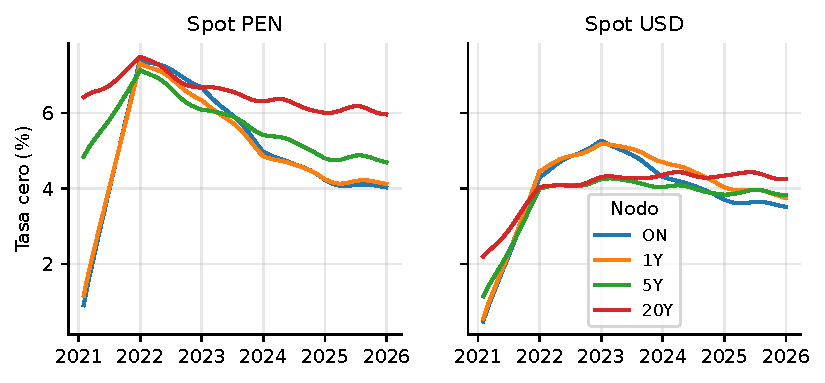
\includegraphics[width=\linewidth]{curvas_spot_historicas.pdf}
  \caption{Curvas spot PEN y USD, 2021--2025 (nodos seleccionados).}\label{fig:curvas}
\end{figure}

\section{Formulación del problema}\label{sec:formulacion}

El problema es una decisión estática: elegir en $t_0$ (31-12-2025) el monto de cada posición de activo y de
pasivo para el horizonte de un año ($t_H$ = 31-12-2026), sin rebalanceo dentro del año. Se optimiza la
estructura conjunta de los seis activos y los seis pasivos existentes; no se considera deuda nueva, porque el
caso asignado no la incluye en su alcance. El Anexo~\ref{app:formulacion} desarrolla la formulación completa y los supuestos en que se apoya.

\subsection{Variables de decisión}
Sea $i$ un activo, $j$ un pasivo y $k$ cualquiera de los doce instrumentos; $z_k$ denota indistintamente
$x_i$ o $y_j$ y $z_k^0$ la posición inicial. Las variables son:

\begin{center}
\begin{tabular}{clll}
\toprule
Variable & Descripción & Dominio & Unidad \\
\midrule
$x_i$ & monto asignado al activo $i$ & $x_i \ge 0$ & S/ mm \\
$y_j$ & monto asignado al pasivo $j$ & $y_j \ge 0$ & S/ mm \\
$\Delta_k^+,\ \Delta_k^-$ & aumento y reducción frente a la posición inicial $z_k^0$ & $\ge 0$ & S/ mm \\
$\zeta$ & valor en riesgo auxiliar (Rockafellar--Uryasev) & libre & S/ mm \\
$u_s$ & exceso de pérdida del escenario $s$ sobre $\zeta$ & $\ge 0$ & S/ mm \\
\bottomrule
\end{tabular}
\end{center}

No hay posiciones cortas: la ausencia de esa alternativa en los datos del caso se traduce en $x_i, y_j \ge 0$.
La reestructuración de cada instrumento se descompone en $z_k - z_k^0 = \Delta_k^+ - \Delta_k^-$, lo que
permite penalizar simétricamente cualquier movimiento, subida o bajada, sin usar variables binarias.

\subsection{Función objetivo}
El resultado del patrimonio y su pérdida en el escenario $s$ son
\begin{equation}
  \Delta \PN_s = \sum_{i} x_i\, r_{i,s} - \sum_{j} y_j\, r_{j,s}, \qquad L_s = -\Delta \PN_s,
\end{equation}
donde $r_{k,s}$ es el resultado a un año del instrumento $k$ bajo el escenario $s$ (Sección~\ref{sec:riesgo}). El
costo de transacción $TC = \sum_k c_k\,(\Delta_k^+ + \Delta_k^-)$, donde $c_k$ es el costo de
reestructuración por sol movido del instrumento $k$ que fija el caso, se aplica igual a subidas y bajadas.
El costo de prepago no se suma a las reducciones de pasivos, porque el caso lo reserva para otros
escenarios de decisión. $TC$ se paga en $t_0$, es determinista y no depende del escenario. El problema es

\begin{equation}
  \max_{x,\,y,\,\Delta,\,\zeta,\,u}\quad \sum_{s} p_s\,\Delta \PN_s \;-\; \lambda\left(\zeta + \frac{1}{1-\alpha}\sum_s p_s\, u_s\right) \;-\; TC
  \qquad\text{s.a. } u_s \ge L_s - \zeta,\ u_s \ge 0.
  \label{eq:objetivo}
\end{equation}

El término entre paréntesis es el $\CVaR_\alpha$ de la pérdida $L_s$ en su forma lineal de
\textcite{rockafellar2000}: minimizarlo sobre $\zeta$ recupera exactamente el valor en riesgo al nivel
$\alpha$ y el promedio de las pérdidas que lo superan. Como el objetivo lo resta, ponderado por la
aversión al riesgo $\lambda \ge 0$, al maximizar el óptimo elige el $\zeta$ que minimiza esa expresión, y la
cola queda penalizada sin perder la linealidad del problema. Con $\lambda = 0$ el objetivo maximiza solo el resultado esperado neto de costos; a medida que
$\lambda$ crece, la solución se acerca a la que minimiza el $\CVaR_{0.95}$ alcanzable (Sección~\ref{sec:resultados}).
El costo de transacción se resta una sola vez, fuera de $L_s$: es un costo cierto de la decisión, no un
riesgo de mercado, de modo que se reporta por separado el patrimonio neto de costos, $\PN_0' = \PN_0 - TC$,
y su valor esperado al horizonte, $\E[\PN_H] = \PN_0' + \E[\Delta \PN]$. La rentabilidad esperada de los
activos es $\sum_s p_s \sum_i x_i r_{i,s} / B_A$ y el costo esperado de los pasivos,
$\sum_s p_s \sum_j y_j r_{j,s} / B_L$. Este es un costo económico: incluye intereses y revalorización.

Dos variantes sirven de comparación. La cartera de \emph{mínima varianza} minimiza
$\sum_s p_s (\Delta \PN_s - \E[\Delta \PN])^2$ sujeta a $\E[\Delta \PN] - TC$ mayor o igual que el de la
cartera óptima y a las mismas restricciones. La variante con \emph{vencimientos exigidos al horizonte}
agrega, para cada grupo de vencimiento remanente, la misma cota de la ecuación~\eqref{eq:pesos} medida con
el plazo que le queda a cada instrumento en $t_H$.

Con probabilidades no uniformes y masas de probabilidad concentradas en unos pocos escenarios de estrés, el
cuantil que define el valor en riesgo puede no ser único cuando $\lambda \to 0$; por eso el $\VaR$ y el
$\CVaR$ que se reportan en los resultados se recalculan \emph{ex post}, sobre la distribución completa de
$\Delta \PN_s$, con la definición de átomo fraccional
$\CVaR_\alpha = \frac{1}{1-\alpha}\big[\sum_{L_s > \VaR} p_s L_s + \VaR\,(1-\alpha - \sum_{L_s > \VaR} p_s)\big]$,
en vez de leer directamente la variable $\zeta$ de la ecuación~\eqref{eq:objetivo}.

\subsection{Restricciones}
Los presupuestos $\sum_i x_i = B_A = 1{,}000$ y $\sum_j y_j = B_L = 800$ (S/ mm) son exógenos y fijan el
denominador de cada peso, de modo que las restricciones del Cuadro~4 del enunciado son lineales en las variables
de decisión: para cada grupo $g$ (moneda, tipo de instrumento, tipo de tasa o vencimiento remanente) y cada
lado $l \in \{A, L\}$,
\begin{equation}
  \underline{w}_g\, B_l \;\le\; \sum_{k \in \mathcal{K}_g} z_k \;\le\; \overline{w}_g\, B_l.
  \label{eq:pesos}
\end{equation}
Un grupo adicional, de concentración, acota individualmente cada instrumento ($z_k \le \overline{w}_g\, B_l$).
Sobre esos límites, el patrimonio neto en $t_0$ debe ser de al menos \PEN120 mm, el cociente pasivos/activos
de a lo más 0.85 y la caja de al menos \PEN80 mm; con los presupuestos fijos, las dos primeras ya se cumplen
por construcción ($\PN_0 = 200$, $P/A = 0.80$) y se mantienen en el modelo solo para que el solver las
verifique y el informe las reporte.

\subsection{Modelo de riesgo}\label{sec:riesgo}
El resultado por instrumento $r_{k,s}$ no se aproxima con una duración o un DV01, sino que se obtiene
revalorizando cada instrumento completo al horizonte bajo el escenario $s$:
\begin{equation}
  r_{k,s} = \frac{V_k^{PEN}(t_H;\,\text{mercado}_s) + CF_k^{PEN}(t_0, t_H]_s}{V_k^{PEN}(t_0)} - 1,
\end{equation}
donde $V_k(t_H)$ es el valor presente de los flujos posteriores a $t_H$ descontados con la curva del
escenario y $CF_k(t_0, t_H]$ son los flujos cobrados o pagados dentro del año, convertidos a soles al tipo de
cambio del escenario en su fecha de pago y sin reinvertir. Como $r_{k,s}$ no depende del tamaño de la
posición, la ecuación~\eqref{eq:objetivo} con esta matriz de resultados fijada de antemano es un problema
lineal.

Los escenarios $s$ combinan dos fuentes, con probabilidad conjunta 95\,\%/5\,\%: 500 trayectorias de un año
obtenidas por remuestreo por bloques de la historia mensual \parencite{kunsch1989}, y los cuatro escenarios de estrés propios del caso, cada uno
con probabilidad 1.25\,\%. El remuestreo concatena dos bloques de seis meses consecutivos de cambios
históricos, en vez de doce meses independientes, para conservar la persistencia mensual documentada en la
Sección~\ref{sec:datos} y no subestimar la varianza anual. A ese shock centrado se le suma una deriva anual que
depende de la clase de factor: nula en las tasas (para no proyectar el ciclo alcista de 2021--2025 hacia
adelante), la paridad de tasas implícita en las curvas de $t_0$ en el tipo de cambio, y el promedio histórico
del log-retorno mensual en la renta variable (aproximadamente 6\,\%/año). En el tipo de cambio, el shock
se desplaza además por una constante para que la media de $FX_H/FX_0$ en la muestra sea exactamente la
forward de paridad. Sumar la paridad al logaritmo sin este ajuste la sobreestima por convexidad
($\E[e^X] = e^{\mu + \sigma^2/2}$) y por el error de muestreo de la media. Dentro del horizonte, cada factor se
mueve linealmente entre su valor en $t_0$ y su valor bajo el escenario en $t_H$, la misma regla con la que se
reproyectan los cupones flotantes que se fijan dentro del año y con la que devenga la caja.

\section{Algoritmo e implementación}\label{sec:algoritmo}

El modelo se resuelve en cinco etapas secuenciales, cada una consumiendo la salida de la anterior.

\textbf{(i) Datos del caso.} Los parámetros del caso asignado (presupuestos, límites del Cuadro~4 del caso, nivel de
confianza, aversión al riesgo, tamaño y semilla del remuestreo) y las posiciones y flujos contractuales
limpios se consolidan en un único documento de entrada, para que ningún límite, costo o posición quede fijado
fuera de esos datos.

\textbf{(ii) Valorización.} Cada instrumento se valora a $t_0$ descontando sus flujos contractuales con la
curva cero de su moneda más un spread calibrado para que ese valor coincida con el valor de mercado
observado, con una tolerancia de $10^{-6}$. La misma función de valorización, con
el mismo spread fijo, revaloriza cada instrumento bajo cualquier escenario de mercado.

\textbf{(iii) Escenarios y riesgo.} Se generan las 504 trayectorias descritas en la Sección~\ref{sec:riesgo} (500
por remuestreo más 4 de estrés) y se revaloriza cada uno de los doce instrumentos bajo cada una, para obtener
la matriz de resultados $r_{k,s}$ que alimenta la optimización. Calcular esa matriz completa toma cerca de un
minuto y se reutiliza en todas las variantes que no cambian los escenarios ni la valorización.

\textbf{(iv) Optimización.} Con $r_{k,s}$ fija, el problema lineal de la ecuación~\eqref{eq:objetivo} se
plantea con \textcite{diamond2016} y se resuelve con el solver de programación lineal de código abierto
HiGHS. La instancia base (12 instrumentos, 504 escenarios y unas 40 restricciones de peso y presupuesto)
converge en 167 iteraciones de simplex y 11 milisegundos. Cuando un grupo de peso queda vacío por la
composición de los instrumentos y su límite inferior es positivo, o cuando los límites de caja o patrimonio
resultan incompatibles entre sí, el problema se declara sin solución en vez de forzar un resultado.

\textbf{(v) Resultados.} La solución óptima, el barrido de la aversión al riesgo $\lambda$, un punto de
comparación de mínima varianza con el mismo resultado neto esperado, el diagnóstico de la posición inicial y
la variante que exige los límites de vencimiento también en el horizonte (Sección~\ref{sec:resultados}) se calculan
en la misma corrida y quedan disponibles como un único registro de resultados: cada cifra, tabla y figura de
este informe se lee directamente de ese registro, sin transcripción manual.

Todo el proceso es reproducible con una semilla fija para el remuestreo. La elección de revalorizar cada
escenario en vez de propagar la matriz de covarianzas de los 24 factores de riesgo (Sección~\ref{sec:datos}) evita
tener que reducir su dimensión: esa matriz es singular y una aproximación lineal exigiría antes una
descomposición de componentes principales o un filtro equivalente, con su propio error de aproximación.

\section{Resultados}\label{sec:resultados}

\subsection{Posición inicial}
Evaluada con el modelo de riesgo de la Sección~\ref{sec:riesgo}, la posición inicial rinde en promedio
$\E[\Delta PN] = \PEN3.96$ mm a un año, con una volatilidad de \PEN25.4 mm y un $\CVaR_{95\%}$ de \PEN50.1 mm
(Cuadro~\ref{tab:riesgo-inicial}): una cuarta parte del patrimonio inicial en el 5\,\% de escenarios más
adversos. Un 25\,\% de esa cola de pérdida proviene de los cuatro escenarios de estrés pese a que representan
solo 1.25\,\% de la probabilidad total, y el escenario de mayor pérdida es una depreciación del sol acompañada
de una caída de tasas y de renta variable, que cuesta \PEN45.6 mm. La única restricción del Cuadro~4 del caso
que la posición inicial incumple es el peso máximo de renta variable en los activos (22\,\% contra 20\,\%).

\begin{table}[htbp]
\centering
\caption{Riesgo a un año de la posición inicial (S/ mm salvo probabilidades).}
\label{tab:riesgo-inicial}
\begin{tabular}{lr}
\toprule
 & valor \\
\midrule
PN0 & 200.00 \\
E[ΔPN] & 3.96 \\
E[PN\_T] & 203.96 \\
σ(ΔPN) & 25.43 \\
VaR 95\% & 42.49 \\
CVaR 95\% & 50.12 \\
P(PN\_T < 120) & 0.00 \\
prob. cola: estrés / total & 0.25 \\
ΔPN C\_STRESS\_1 & -1.03 \\
ΔPN C\_STRESS\_2 & -45.61 \\
ΔPN C\_STRESS\_3 & -23.34 \\
ΔPN C\_STRESS\_4 & -8.50 \\
\bottomrule
\end{tabular}
\end{table}


\subsection{Cartera óptima}
Con la aversión al riesgo de referencia del caso, $\lambda = 0.25$, la reasignación óptima
(Cuadro~\ref{tab:posiciones-optimas} y Figura~\ref{fig:posiciones}) concentra los activos en soles: la caja
sube a \PEN200 mm (el máximo de 20\,\% de los activos, no el piso de \PEN80 mm, que queda muy por debajo) y el
bono fijo en soles A02 sube a su tope individual de \PEN350 mm. Del lado en dólares, el bono flotante A05 casi
se duplica a \PEN240 mm mientras que el bono fijo A04 se liquida por completo; la renta variable A06 cae a su
piso implícito de 5\,\% (\PEN50 mm), el mínimo compatible con los máximos de caja y renta fija. En los pasivos,
el préstamo corto en soles L01 sube a su tope de concentración (\PEN280 mm) y el bono fijo L02 baja a
\PEN40 mm, mientras que la mezcla de tasa fija y flotante de los pasivos queda exactamente en sus dos límites
(45\,\% fijo, 55\,\% flotante): son restricciones gemelas, extremos opuestos de la misma partición.

\begin{table}[htbp]
\centering
\caption{Posiciones inicial, óptima (λ = 0.25) y alternativas (S/ mm).}
\label{tab:posiciones-optimas}
\resizebox{\ifdim\width>\textwidth\textwidth\else\width\fi}{!}{%
\begin{tabular}{llllrrrrr}
\toprule
 & Lado & Instrumento & Moneda & Inicial & Óptimo (λ = 0.25) & Cambio & Media-varianza & Vencimientos en t\_H (ENFORCE) \\
\midrule
A01 & Activo & Caja PEN & PEN & 150.0 & 200.0 & 50.0 & 194.7 & 200.0 \\
A02 & Activo & Bono PEN Fijo 2030 & PEN & 180.0 & 350.0 & 170.0 & 350.0 & 350.0 \\
A03 & Activo & Bono PEN Flotante 2031 & PEN & 160.0 & 160.0 & 0.0 & 200.1 & 160.0 \\
A04 & Activo & Bono USD Fijo 2032 & USD & 150.0 & 0.0 & -150.0 & 0.0 & 0.0 \\
A05 & Activo & FRN USD 2030 & USD & 140.0 & 240.0 & 100.0 & 199.9 & 240.0 \\
A06 & Activo & ETF renta variable global & USD & 220.0 & 50.0 & -170.0 & 55.3 & 50.0 \\
L01 & Pasivo & Préstamo PEN CP flotante & PEN & 120.0 & 280.0 & 160.0 & 273.1 & 200.0 \\
L02 & Pasivo & Bono PEN Fijo 2029 & PEN & 150.0 & 40.0 & -110.0 & 40.0 & 103.7 \\
L03 & Pasivo & Bono PEN Fijo 2036 & PEN & 180.0 & 180.0 & 0.0 & 180.0 & 158.2 \\
L04 & Pasivo & Préstamo PEN Flotante 2032 & PEN & 110.0 & 110.0 & 0.0 & 110.0 & 110.0 \\
L05 & Pasivo & Bono USD Fijo 2031 & USD & 140.0 & 140.0 & 0.0 & 140.0 & 140.0 \\
L06 & Pasivo & Préstamo USD Flotante 2035 & USD & 100.0 & 50.0 & -50.0 & 56.9 & 88.0 \\
\bottomrule
\end{tabular}}
\end{table}


\begin{figure}[htbp]\centering
  \caption{Posiciones inicial y óptima por instrumento (barras) y de la variante con vencimientos exigidos en
  $t_H$ (marca horizontal).}\label{fig:posiciones}
  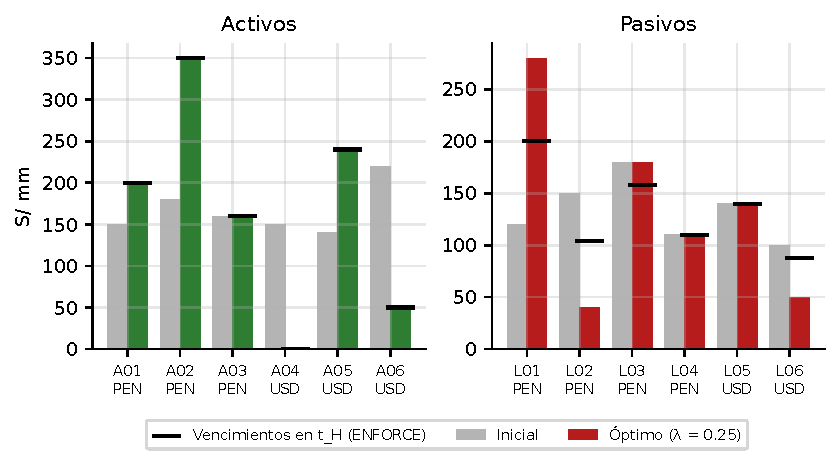
\includegraphics[width=\linewidth]{posiciones_inicial_optima.pdf}
\end{figure}

Esa reasignación paga \PEN2.73 mm en costos de transacción y sube el resultado esperado bruto a
\PEN5.83 mm; aun así, el resultado neto (\PEN3.11 mm) queda por debajo del de la posición inicial
(\PEN3.96 mm). El modelo cede \PEN0.85 mm de valor esperado a cambio de bajar la volatilidad del patrimonio
de \PEN25.4 mm a \PEN7.0 mm y el $\CVaR_{95\%}$ de \PEN50.1 mm a \PEN7.8 mm, una caída de 84\,\%
(Cuadro~\ref{tab:metricas-optimizacion}). La rentabilidad esperada de los activos apenas cambia (de 6.08\,\% a
6.01\,\%), pero el costo esperado de los pasivos baja de 7.10\,\% a 6.79\,\%: la ganancia de la optimización
viene sobre todo de una estructura de pasivos más barata y menos expuesta a la cola, no de activos más
rentables.

\begin{table}[htbp]
\centering
\caption{Métricas a un año (S/ mm salvo indicación). α = 0.95; objetivo evaluado con λ = 0.25.}
\label{tab:metricas-optimizacion}
\resizebox{\ifdim\width>\textwidth\textwidth\else\width\fi}{!}{%
\begin{tabular}{lrrrr}
\toprule
 & Inicial & Óptimo (λ = 0.25) & Media-varianza & Venc. exigidos al horizonte \\
\midrule
Objetivo (E − λ·CVaR − TC) & -9.34 & 0.91 & 0.70 & 0.70 \\
E[ΔPN] & 3.29 & 5.56 & 5.55 & 4.53 \\
Costo de transacción & 0.00 & 2.72 & 2.71 & 1.83 \\
E[ΔPN] − TC & 3.29 & 2.84 & 2.84 & 2.70 \\
E[PN] al horizonte & 203.29 & 202.84 & 202.84 & 202.70 \\
σ(ΔPN) & 25.33 & 6.27 & 5.74 & 5.66 \\
VaR 95 \% & 43.07 & 3.88 & 3.06 & 2.78 \\
CVaR 95 \% & 50.52 & 7.71 & 8.55 & 8.02 \\
Rentabilidad esperada activos (\%) & 5.95 & 5.94 & 5.94 & 5.94 \\
Costo esperado pasivos (\%) & 7.02 & 6.73 & 6.73 & 6.86 \\
Estrés en la cola (\%) & 25.00 & 25.00 & 25.00 & 25.00 \\
Pérdida C\_STRESS\_1 & 1.03 & -13.30 & -5.07 & -11.84 \\
Pérdida C\_STRESS\_2 & 45.61 & 13.90 & 19.85 & 20.35 \\
Pérdida C\_STRESS\_3 & 23.34 & -13.02 & -2.21 & -6.51 \\
Pérdida C\_STRESS\_4 & 8.50 & -19.84 & -12.75 & -21.99 \\
\bottomrule
\end{tabular}}
\end{table}


\subsection{Barrido de la aversión al riesgo}
Variar $\lambda$ entre 0 y 5 traza la frontera entre resultado esperado neto y $\CVaR_{95\%}$
(Cuadro~\ref{tab:barrido-lambda} y Figura~\ref{fig:frontera}). Con $\lambda = 0$ el objetivo ignora el riesgo y
elige una solución de esquina: 49\,\% de activos en dólares y 20\,\% en renta variable, con un
$\CVaR_{95\%}$ de \PEN61.0 mm, más riesgosa que la propia posición inicial. Subir $\lambda$ a 0.1 ya recorta
ese CVaR a \PEN32.1 mm, y en $\lambda = 0.25$ la solución colapsa a los límites de caja y renta fija descritos
arriba. Para $\lambda \ge 0.5$ el resultado esperado neto cae por debajo de \PEN1.1 mm y en $\lambda = 5$ se
vuelve negativo (\mbox{$-$\PEN0.69} mm): a partir de ahí, evitar más cola cuesta más de lo que queda de
resultado esperado. La composición de la cartera se mueve en la misma dirección: la renta variable salta del
20\,\% al piso de 5\,\% no bien $\lambda$ deja de ser cero, y el peso de pasivos en dólares sube de 23.75\,\%
a 43\,\% a medida que $\lambda$ crece, porque financiarse en dólares resulta, en este conjunto de escenarios,
más barato en la cola que financiarse en soles.

\begin{table}[htbp]
\centering
\caption{Barrido de λ: resultado esperado, costo, riesgo y composición (S/ mm y \% del lado).}
\label{tab:barrido-lambda}
\resizebox{\ifdim\width>\textwidth\textwidth\else\width\fi}{!}{%
\begin{tabular}{lrrrrrrrrr}
\toprule
 & E[ΔPN] & TC & E[ΔPN] − TC & σ(ΔPN) & CVaR 95 \% & Activos USD (\%) & Equity (\%) & Pasivos USD (\%) & Pasivos flotantes (\%) \\
\midrule
0.000000 & 9.15 & 2.31 & 6.84 & 30.22 & 60.97 & 49.00 & 20.00 & 23.75 & 55.00 \\
0.100000 & 8.26 & 2.17 & 6.09 & 19.79 & 32.06 & 41.00 & 17.00 & 20.00 & 47.60 \\
0.250000 & 5.83 & 2.73 & 3.11 & 7.03 & 7.82 & 29.00 & 5.00 & 23.75 & 55.00 \\
0.500000 & 7.26 & 6.13 & 1.12 & 5.96 & 2.54 & 27.46 & 5.00 & 27.63 & 52.13 \\
1.000000 & 7.41 & 6.62 & 0.79 & 6.09 & 2.01 & 28.35 & 5.00 & 28.56 & 51.06 \\
2.000000 & 7.62 & 7.61 & 0.01 & 5.91 & 1.52 & 33.73 & 5.00 & 35.37 & 53.45 \\
5.000000 & 7.96 & 8.66 & -0.69 & 6.02 & 1.35 & 40.00 & 5.00 & 43.11 & 55.00 \\
\bottomrule
\end{tabular}}
\end{table}


\begin{figure}[htbp]\centering
  \caption{Frontera resultado esperado neto vs. $\CVaR_{95\%}$ sobre el barrido de $\lambda$, con la posición
  inicial, el punto de comparación de mínima varianza y la variante con vencimientos exigidos en $t_H$.}
  \label{fig:frontera}
  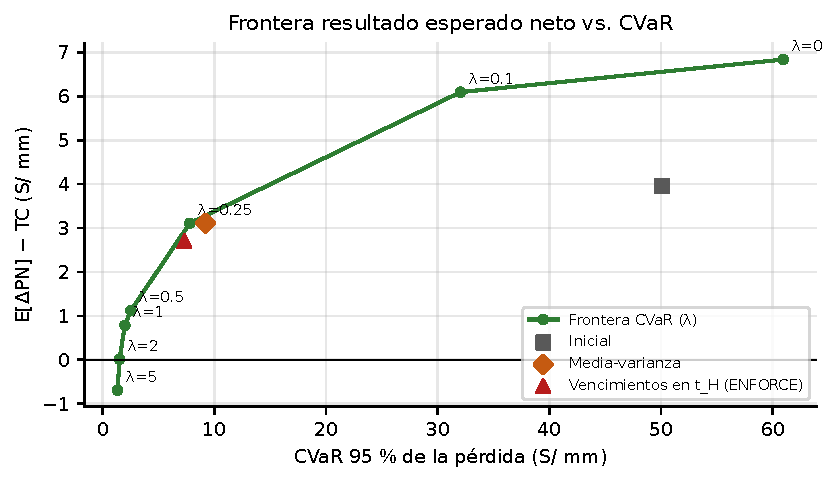
\includegraphics[width=0.65\linewidth]{frontera_lambda.pdf}
\end{figure}

\subsection{Comparación con mínima varianza y con vencimientos exigidos en el horizonte}
Fijando el mismo resultado esperado neto que la cartera óptima (\PEN3.11 mm), una cartera de mínima varianza
con las mismas restricciones logra una volatilidad algo menor (\PEN6.40 mm contra \PEN7.03 mm) pero un
$\CVaR_{95\%}$ mayor (\PEN9.23 mm contra \PEN7.82 mm): optimizar directamente la medida de riesgo que exige el
caso controla mejor la cola que minimizar la dispersión total, aunque acepte algo más de varianza en el
centro de la distribución. Exigir que los límites de vencimiento del Cuadro~4 del caso se cumplan también en $t_H$, y no solo en $t_0$ como
hace la solución base, cuesta \PEN0.29 mm de objetivo (de 1.16 a 0.87). El préstamo corto L01 baja de
\PEN280 mm a \PEN200 mm y el $\CVaR_{95\%}$ mejora a \PEN7.33 mm, porque esa restricción adicional también
limita, de paso, la concentración de la cartera óptima base.

\begin{figure}[htbp]\centering
  \caption{Distribución de $\Delta PN$ a un año: posición inicial, cartera óptima y mínima varianza
  (histograma: escenarios de remuestreo; triángulos: escenarios de estrés; línea punteada: $-\CVaR_{95\%}$ de
  cada cartera).}\label{fig:distribucion-optima}
  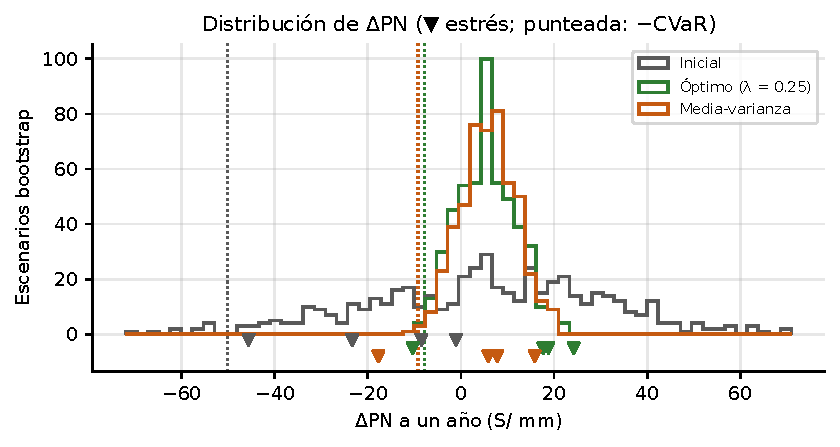
\includegraphics[width=0.75\linewidth]{distribucion_dpn_optima.pdf}
\end{figure}

La Figura~\ref{fig:distribucion-optima} resume el efecto conjunto: la distribución de la cartera óptima es
mucho más angosta que la inicial y sus escenarios de estrés, que en la posición inicial caían muy por debajo
del grueso de la distribución, quedan cerca del cuerpo de la distribución remuestreada.

\section{Validación y análisis de sensibilidad}\label{sec:sensibilidad}
% Pruebas (Anexo C), cambios en lambda, tasas (+200 pb cortas), límites y costos.
\todo{Sensibilidades del caso.}

\section{Opinión del analista}\label{sec:opinion}

El modelo tiene tres fortalezas que valen su costo computacional. Primero, revalorizar cada instrumento por
sus flujos completos, en vez de aproximar con duración o DV01, es lo que permite detectar que el riesgo de
tasa corta de la cartera óptima cambia de signo según la convención de proyección de cupones flotantes
(Sección~\ref{sec:sensibilidad}); una aproximación lineal habría escondido ese riesgo de modelo. Segundo, linealizar
el CVaR con la formulación de Rockafellar--Uryasev mantiene el problema como programa lineal, resoluble en
milisegundos, sin perder la coherencia entre el CVaR que entra en el objetivo y el que se reporta \emph{ex
post}. Tercero, la batería de nueve sensibilidades (tasas, precios sombra, costos, confianza, peso de la
cola, semilla, deriva, sesgo del estrés y regla de cupones) obliga a distinguir qué parte del resultado viene
de la optimización y qué parte viene de supuestos que el enunciado del caso no fija por completo.

Esa misma batería expone las debilidades del modelo. El conjunto de estrés castiga solo una dirección del
tipo de cambio: los cuatro escenarios deprecian el sol. Buena parte de la preferencia de la cartera
óptima por activos en dólares depende de esa asimetría (apartado~\ref{subsec:sesgo-estres}), y un comité de riesgos debería incorporar un
escenario de apreciación del sol al conjunto base, no solo como sensibilidad. El remuestreo por bloques
reproduce bien la razón de varianzas a 12 meses observada en la historia, pero esa historia cubre cinco años y
un solo ciclo de alza de tasas; la prueba de semillas alternativas muestra una dispersión de CVaR de
\PEN5.6 mm a \PEN7.7 mm que, sin ser grande, tampoco es despreciable frente al \PEN7.82 mm de la base. Y la
convención de proyección de cupones flotantes (nivel plano del factor de referencia frente a forward del
período) no está fijada de manera inequívoca por los datos del caso y cambia materialmente el resultado en
el escenario de estrés más severo; este informe la trata como una sensibilidad porque no hay evidencia
suficiente para preferir una convención sobre la otra, pero es la fuente de riesgo de modelo más grande de
todo el análisis.

Con más tiempo o más datos, extendería la historia de mercado más allá de cinco años para cubrir más de un
ciclo de tasas, y adoptaría como cartera base la variante que exige los límites de vencimiento también en el
horizonte: la solución base los incumple con certeza en el préstamo corto L01, y corregirlo cuesta solo
\PEN0.29 mm de resultado esperado neto. También agregaría de forma permanente al conjunto de estrés un
escenario de apreciación del sol, en vez de dejarlo como sensibilidad aparte, para que la cartera recomendada
no dependa de la dirección cambiaria de los cuatro escenarios que trae el caso.


\printbibliography

\clearpage
\appendix
\section{Instrucciones de ejecución}\label{app:instrucciones}
Requiere Python $\ge$ 3.11 y \texttt{uv}; el informe se compila con LuaLaTeX (\texttt{latexmk}).
\begin{lstlisting}[language=bash]
make setup        # .venv con el paquete en modo editable
make all          # Excel -> tablas limpias -> input.json -> output.json
make sensitivity  # sensibilidades S1-S9 -> sensitivity.json (5-8 min)
make test         # pruebas automaticas (Anexo C)
make notebooks    # ejecuta los notebooks: tablas y figuras del informe
make report       # compila el informe
\end{lstlisting}
Sin \texttt{make}, los mismos pasos son \texttt{python -m optimum \{data,json,run,sensitivity\}}. Todos los
parámetros (límites, $\lambda$, $\alpha$, costos, semilla y escenarios) se leen de \texttt{data/json/input.json}.

\section{Uso de inteligencia artificial}\label{app:ia}
% Fuente: docs/ia/ (registro automático de prompts + decisiones + errores detectados).
% `python scripts/ia_log_to_tex.py` genera appendices/B_prompts_generado.tex.

\subsection{Herramientas y forma de trabajo}
\todo{Claude Code con skills y hooks del proyecto (.claude/).}

\subsection{Errores y simplificaciones de la IA corregidos (mínimo 2)}
\begin{enumerate}
  \item \todo{Error 1: qué propuso la IA, cómo se detectó, cómo se corrigió.}
  \item \todo{Error 2.}
\end{enumerate}

\subsection{Prompts principales}
\IfFileExists{appendices/B_prompts_generado.tex}{% Generado por scripts/ia_log_to_tex.py — no editar a mano
\begin{description}
\item[P01 · 2026-09-27 · Estructura del proyecto] \hfill\\
\textit{Prompt:} Estructurar un proyecto Python con notebooks, datos crudos/intermedios/procesados, utilidades de figuras, informe LaTeX con Docker y un espacio para Claude Code con skills y arneses.\\
\textit{Resultado:} Aceptado\\
\textit{Detalle:} Se generó el andamiaje, el pipeline de limpieza con validaciones y el contrato JSON. La lógica financiera (valorización, riesgo, optimizador) quedó sin implementar a propósito.\\
\item[P02 · 2026-09-27 · uv, git init y corrección del caso asignado] \hfill\\
\textit{Prompt:} \enquote{usemos uv para el proyecto}; \enquote{inicializa git}; \enquote{El caso que me toca resolver es el C}.\\
\textit{Resultado:} Aceptado\\
\textit{Detalle:} \texttt{make setup} pasó a \texttt{uv}; se inicializó git. Se corrigió el caso asignado a C.\\
\item[P03 · 2026-09-27 · Formulación base del Caso C (CVaR)] \hfill\\
\textit{Prompt:} \enquote{Dado que me tocó el caso C, cómo debo empezar}; \enquote{qué me recomiendas para la formulación}; \enquote{qué otras maneras hay de formularlo}; \enquote{vamos con lo acordado (versión base)}.\\
\textit{Resultado:} Aceptado\\
\textit{Detalle:} La IA propuso un LP con CVaR (Rockafellar–Uryasev) sobre resultados por revalorización completa, más alternativas; el alumno eligió la versión base (D-06 a D-12). El auditor halló los errores E01–E03.\\
\item[P04 · 2026-09-27 · Valorizador por flujos (valuation.py)] \hfill\\
\textit{Prompt:} \enquote{sigamos con la valorización, muéstrame el plan}; \enquote{sí, vamos con (a), escribe los tests}; \enquote{sí, implementa valuation.py}.\\
\textit{Resultado:} Aceptado\\
\textit{Detalle:} Plan, 18 pruebas antes del código e implementación de \texttt{valuation.py}. V0 = valor de mercado en los 12 instrumentos; flotantes con proyección plana (D-13).\\
\item[P05 · 2026-09-27 · Cierre de los notebooks 00, 01 y 02] \hfill\\
\textit{Prompt:} \enquote{y los notebooks en que momento se realiza?}; \enquote{cierra primero los notebooks 00, 01 y 02}.\\
\textit{Resultado:} Aceptado\\
\textit{Detalle:} Cierre de los notebooks 00–02 sin lógica fuera de \texttt{src/}. La IA corrigió una frase propia que atribuía sin verificar la diferencia de spreads a la convención de días.\\
\item[P06 · 2026-09-28 · Modelo de riesgo (risk.py) y notebook 03] \hfill\\
\textit{Prompt:} \enquote{vamos con el plan de risk}; \enquote{estoy de acuerdo con las recomendaciones}; \enquote{continuemos con la implementación}.\\
\textit{Resultado:} Aceptado con corrección\\
\textit{Detalle:} Plan, decisiones D-14 a D-16, 29 pruebas y \texttt{risk.py} (504 escenarios). La IA detectó un sesgo de media en su bootstrap (E04) y se centraron las ventanas (D-09 v3). Posición inicial: VaR95 = 42.5, CVaR95 = 50.1 S/ mm.\\
\item[P07 · 2026-09-28 · Auditoría de la capa (iii) y correcciones] \hfill\\
\textit{Prompt:} \enquote{lanza la auditoria}; elección de la regla de transición del estrés (dos rondas).\\
\textit{Resultado:} Aceptado con corrección\\
\textit{Detalle:} Auditoría sin errores críticos. Hallazgos sobre la transición del estrés (E05, D-11 v2), riesgo de modelo de D-13 y sesgo de los estrés hacia USD; 14 pruebas nuevas. VaR y CVaR sin cambio.\\
\item[P08 · 2026-09-28 · Lectura del notebook 03] \hfill\\
\textit{Prompt:} \enquote{agrega la lectura al notebook}.\\
\textit{Resultado:} Aceptado con corrección\\
\textit{Detalle:} Borrador de lectura del notebook 03. Antes de entregarlo, la IA corrigió tres afirmaciones; la principal: la cola del bootstrap es el régimen de 2022 (tasas al alza), no una caída de tasas.\\
\item[P09 · 2026-09-28 · Optimizador (optimizer.py): plan, pruebas primero e implementación] \hfill\\
\textit{Prompt:} \enquote{vamos con el plan del optimmizer}; \enquote{dale, usa el generador-pruebas}; \enquote{dale, implementa}.\\
\textit{Resultado:} Aceptado\\
\textit{Detalle:} Plan del optimizador (LP R–U y benchmark media-varianza). La IA preguntó las ambigüedades (D-18, D-19, LE\_12M). \texttt{generador-pruebas} escribió 44 casos sin ver el código; la implementación pasó las 123 pruebas.\\
\item[P10 · 2026-09-28 · Auditoría del optimizador y límites al horizonte] \hfill\\
\textit{Prompt:} \enquote{o es mejor primero ejecutar el auditor financiero para saber que hacer?}; decisiones del alumno sobre LE\_12M, reporte al horizonte y sensibilidad D-13.\\
\textit{Resultado:} Aceptado con corrección\\
\textit{Detalle:} El alumno propuso auditar antes de decidir LE\_12M. La auditoría halló el reporte al horizonte incompleto (E06); se eligió base con reporte más variante ENFORCE (D-20).\\
\item[P11 · 2026-09-28 · Notebook 04 (optimización)] \hfill\\
\textit{Prompt:} \enquote{vamos con el notebook 04}.\\
\textit{Resultado:} Aceptado (lectura pendiente de validación del alumno)\\
\textit{Detalle:} Notebook 04: 4 figuras, 5 tablas y verificación de que E[ΔPN] y CVaR de \texttt{output.json} se reproducen. Lectura pendiente de validación del alumno.\\
\item[P12 · 2026-09-28 · Sensibilidades S1-S9: formulación, pruebas primero e implementación] \hfill\\
\textit{Prompt:} \enquote{propón las sensibilidades}; \enquote{dale, implementa}.\\
\textit{Resultado:} Aceptado (el alumno eligió evaluación instantánea para ±200 pb, switch de cupones, salida separada y estrés espejo)\\
\textit{Detalle:} Nueve sensibilidades (S1–S9, D-21, D-22) con 23 pruebas antes del código. S2 solo reporta cotas de peso porque el dual del presupuesto no coincide con subir \$B\_A\$.\\
\item[P13 · 2026-09-28 · Notebook 05 (resultados y sensibilidad)] \hfill\\
\textit{Prompt:} \enquote{haz el commit y vamos con el notebook 05\_resultados\_sensibilidad}.\\
\textit{Resultado:} Aceptado (lectura pendiente de validación del alumno)\\
\textit{Detalle:} Notebook 05 sobre \texttt{sensitivity.json} y \texttt{output.json}, sin recalcular. Robustos: cobertura PEN y CVaR; frágiles: posición USD y resultado esperado. Lectura pendiente de validación.\\
\item[P14 · 2026-09-28 · Revisión final: auditoría, revisión del informe y correcciones] \hfill\\
\textit{Prompt:} \enquote{Antes de escribir los anexos, lancemos el auditor financiero y también el revisor del informe}; \enquote{a, corrígelo en el código y sigue con el plan}.\\
\textit{Resultado:} Corregido (el alumno eligió corregir la deriva FX en el código en vez de documentarla como supuesto)\\
\textit{Detalle:} Auditor y revisor hallaron un parámetro fijo en \texttt{cleaning.py}, el sesgo de la deriva FX (E08) y cifras mal leídas (E09). Se corrigió en el código (D-24) y se reescribió el informe.\\
\item[P15 · 2026-09-30 · Notebook de entrega autocontenido] \hfill\\
\textit{Prompt:} \enquote{Lo que realmente se va a subir como zip va a ser el informe, el input.json, el output.json y un notebook que reciba el input lo procese y nos de el output. Para ello condensa todo lo necesario del proyecto en un nuevo notebook...}\\
\textit{Resultado:} Aceptado\\
\textit{Detalle:} Notebook de entrega generado desde \texttt{src/} por script (D-25). Ejecutado aislado, reprodujo \texttt{output.json}; una prueba lo mantiene al día y \texttt{make entrega} arma el zip.\\
\item[E01 · 2026-09-27 · Bootstrap i.i.d. de 12 meses (D-09)] \hfill\\
\textit{Prompt:} Formulación base del Caso C.\\
\textit{Resultado:} Corregido\\
\textit{Detalle:} La IA sumó 12 meses i.i.d. y descartó el bootstrap por bloques con un argumento falso. La autocorrelación (0.94–0.96) hace que el i.i.d. subestime la dispersión anual. Lo detectó el auditor.\\
\item[E02 · 2026-09-27 · Doble cobro de costos al reducir pasivos (D-08)] \hfill\\
\textit{Prompt:} Formulación base del Caso C.\\
\textit{Resultado:} Corregido\\
\textit{Detalle:} Cada reducción de pasivos pagaba restructuring y prepago a la vez. Lo detectó el auditor; se aplica solo el costo que corresponde a cada caso.\\
\item[E03 · 2026-09-27 · Justificación inexacta del centrado (S1) y tratamiento asimétrico de la tasa corta] \hfill\\
\textit{Prompt:} Formulación base del Caso C.\\
\textit{Resultado:} Corregido\\
\textit{Detalle:} Justificó mal el centrado (el carry no explica E[ΔPN]) y trató asimétricamente la tasa corta de la caja y los flotantes, sesgando contra la deuda flotante. Lo detectó el auditor.\\
\item[E04 · 2026-09-28 · Centrado mensual en un bootstrap por bloques (D-09 v3)] \hfill\\
\textit{Prompt:} \enquote{continuemos con la implementación} (risk.py).\\
\textit{Resultado:} Corregido\\
\textit{Detalle:} Asumió que centrar los cambios mensuales daba media cero en el bootstrap por bloques; no es así (+1.2 \% en equity). Se vio al revisar resultados y se centraron las ventanas, con 2 tests nuevos.\\
\item[E05 · 2026-09-28 · Justificación falsa de la transición del estrés (D-11 v2)] \hfill\\
\textit{Prompt:} Formulación base (D-11) y respuesta a la auditoría I-1.\\
\textit{Resultado:} Corregido\\
\textit{Detalle:} Justificó la transición del estrés con un argumento falso y recomendó una alternativa sin calcularla. El auditor lo mostró, la IA lo verificó antes de programar y el alumno eligió interpolar t·s(t).\\
\item[E06 · 2026-09-28 · Reporte al horizonte incompleto y plazos por días/365 en el optimizador] \hfill\\
\textit{Prompt:} \enquote{dale, implementa} (optimizer.py).\\
\textit{Resultado:} Corregido\\
\textit{Detalle:} Revisaba al horizonte solo los grupos MATURITY y medía plazos en días/365. Se reportan todos los grupos con tenencias en t\_H y se usan meses calendario (D-20).\\
\item[E07 · 2026-09-28 · Cifras de estrés mal atribuidas y precios sombra engañosos] \hfill\\
\textit{Prompt:} \enquote{vamos con el notebook 04}; \enquote{propón las sensibilidades} / \enquote{dale, implementa}.\\
\textit{Resultado:} Corregido\\
\textit{Detalle:} Atribuyó a la cartera base cifras de estrés de la reoptimizada y relajó por separado cotas gemelas en S2, lo que sugería costo cero. Se corrigió el texto y se relajan juntas (D-23).\\
\item[E08 · 2026-09-28 · Deriva FX por paridad sin corrección de convexidad (D-24)] \hfill\\
\textit{Prompt:} Formulación base (D-06 v2) e implementación de risk.py.\\
\textit{Resultado:} Corregido\\
\textit{Detalle:} La deriva FX por paridad omitía la convexidad (≈ 25 pb/año a favor de estar largo en USD). El test no lo detectaba. Se corrigió con \texttt{risk.match\_forward} (D-24).\\
\item[E09 · 2026-09-28 · Cifras del informe mal leídas de las tablas] \hfill\\
\textit{Prompt:} \enquote{Vamos a escribir el informe...}; \enquote{/humaniser hay que reescribir el informe...}.\\
\textit{Resultado:} Corregido\\
\textit{Detalle:} En el informe, la IA leyó mal ocho cifras de los JSON (signos, rotación, escenario más severo, entre otras). Los subagentes las detectaron y se contrastó cada cifra con el JSON.\\
\end{description}
}{\todo{Generar con scripts/ia\_log\_to\_tex.py}}

\section{Pruebas automáticas}\label{app:pruebas}
La batería (\texttt{make test}) tiene 167 casos en \texttt{tests/}, y todos pasan con los datos entregados.
La mayoría se escribió a partir de \texttt{docs/formulacion.md}, antes de implementar cada capa, con
resultados calculados a mano. El Cuadro~\ref{tab:pruebas} resume las que pide el enunciado y las que más
protegen la validez del modelo.

\begin{table}[htbp]
\centering\small
\caption{Pruebas principales: qué verifican y resultado.}\label{tab:pruebas}
\begin{tabular}{p{0.28\textwidth}p{0.55\textwidth}l}
\toprule
Prueba (archivo) & Qué verifica & Resultado \\
\midrule
Caso simple resuelto a mano (\texttt{test\_optimizer})
  & Balance de juguete (dos activos, un pasivo, cinco escenarios). La solución analítica con $\lambda=0.5$
    (caja 60, bono 40, pasivo 80; objetivo 0.112) se reproduce con tolerancia $10^{-6}$.
  & pasa \\
CVaR del LP = CVaR \emph{ex post} (\texttt{test\_optimizer})
  & Para varios $\alpha$ y $\lambda$, $\zeta+\sum p_s u_s/(1-\alpha)$ coincide con el CVaR recalculado con
    átomo fraccional, incluido el caso en que el VaR cae dentro de un átomo de probabilidad.
  & pasa \\
Cambio extremo de tasas (\texttt{test\_optimizer})
  & Con $+500$ pb en los nodos cortos de ambas curvas en todos los escenarios, la solución se mueve en la
    dirección esperada. La exposición neta a la tasa corta (caja y activos indexados al tramo corto, menos
    los pasivos indexados a él) sube al menos \PEN1 mm; los activos cortos no bajan y los pasivos cortos no
    suben.
  & pasa \\
Restricciones infactibles (\texttt{test\_optimizer})
  & Tres contradicciones: renta variable máxima bajo su piso implícito, caja mínima sobre la máxima y
    mínimos de moneda que suman 110\,\%. En los tres, el programa informa \texttt{INFEASIBLE} sin lanzar una
    excepción y con un \texttt{output.json} válido.
  & pasa \\
Sin parámetros en el código (\texttt{test\_optimizer}, \texttt{test\_cleaning})
  & Si se cambian en \texttt{input.json} la concentración máxima, $\lambda$, los costos o las
    probabilidades de estrés, la solución cambia o el programa sigue funcionando.
  & pasa \\
Valorización a mano (\texttt{test\_valuation})
  & Cero cupón y bono de dos flujos con interpolación calculados a mano; calibración con $V_0$ igual al
    valor de mercado ($10^{-6}$); forwards recalculadas iguales a las del Excel; flotantes sin
    información futura.
  & pasa \\
Escenarios (\texttt{test\_risk})
  & Bootstrap de juguete con ventanas centradas; deriva sumada solo al bootstrap; media muestral de
    $FX_T/FX_0$ igual a la forward de paridad (D-24); estrés con transición $t\,s(t)$; $\sum p_s = 1$.
  & pasa \\
Monotonía en $\lambda$ y costos (\texttt{test\_optimizer}, \texttt{test\_sensitivity})
  & Al subir $\lambda$, el CVaR y el resultado esperado no suben. Con costos más altos el objetivo no sube.
    Con costo cero la rotación no es menor.
  & pasa \\
Horizonte (\texttt{test\_optimizer})
  & Incumplimientos al horizonte calculados a mano. El de vencimiento a 12 meses es determinista, y la
    variante \texttt{ENFORCE} lo impone.
  & pasa \\
\bottomrule
\end{tabular}
\end{table}

\end{document}
